\subsection{Analog-to-Digital Converter (ADC)}

To measure the phase currents once per PWM cycle an ADC is used. The Zynq has two 12 bit ADCs which enables it to sample two signals simultaneously. It is important to sample the input signals same time to avoid distortion by having a small time delay between current samples. 

Due to the symmetry between the three phases only two of the phases needs to be measured and the last can be caltulated with equation \ref{eq:third_phase}.
\begin{equation}
    I_C = -(I_A + I_B)
    \label{eq:third_phase}
\end{equation}
The calculation of the last phase is done in the processing system.

To control the ADC the IP block \textit{XADC} is used which can be seen on figure \ref{fig:adc_module}. 

\begin{figure}[H]
	\centering
	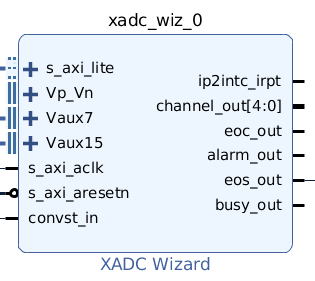
\includegraphics[width=0.35\textwidth]{pictures/software/adc.png}
	\caption{}
	\label{fig:adc_module}
\end{figure}

The block is configured to be triggered by an external signal which is connected to one of the ADC pulses produced by a PWM module.

The signal end-of-sequence, \textit{eos\textunderscore out}, outputs a pulse when a conversion has ended. The signal is used to trigger the interrupt on the processing system as can be seen on figure \ref{fig:adc_block_diagram}.

\begin{figure}[H]
	\centering
	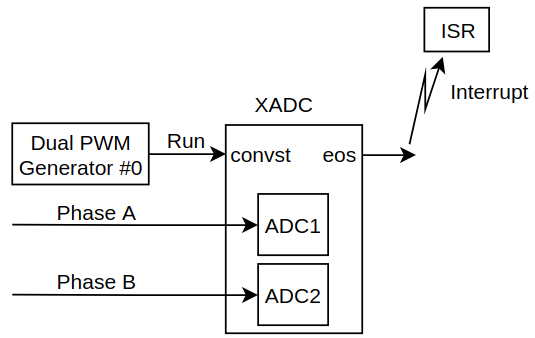
\includegraphics[width=0.5\textwidth]{pictures/software/adc_block_diagram.png}
	\caption{}
	\label{fig:adc_block_diagram}
\end{figure}



